\documentclass[authordate, empirical]{jote-new-article}

\usepackage{caption}

\usepackage{tabularx}

\usepackage{graphicx}

\usepackage{hyperref}

\usepackage[backend=biber,style=apa]{biblatex}

\addbibresource{bibliography.bib}

\jotetitle{Empathic Accuracy, Mindfulness, and Facial Emotion Recognition: An Experimental Study}
\keywordsabstract{emotion recognition, empathic accuracy, facial expressions, interpersonal, mindfulness}
\abstracttext{\textbf{Background and Objectives:} Empathic accuracy, i.e., the degree to which one is able to accurately infer the emotions of others, may be acutely malleable. We examined this idea by testing the immediate effect of a brief mindfulness intervention or facial emotion recognition training.
\textbf{Methods:} Participants were English- or Dutch-speaking psychology students who were assigned to one of three brief intervention conditions (all instructions given in English): (1) verbal instructions for practicing awareness of their body (mindfulness, n = 23); (2) verbal and visual instructions regarding the detection of visual cues for anger, fear, sadness, and happiness (facial emotion recognition training, n = 23); or (3) a verbal, neutral didactic lecture on mindfulness (control, n = 23). Subsequently, participants completed a Dutch-language empathic accuracy task.
\textbf{Results:} There was no significant overall difference in empathic accuracy between the three participant subgroups, suggesting no effect of the two target interventions. Nonetheless, even though empathic accuracy appeared unaltered by facial emotion recognition training among participants who understood Dutch well, it was better after this intervention than after the control intervention among participants with a relatively limited understanding of Dutch.
\textbf{Limitations:} The study used a small convenience sample. The control condition was listening to a lecture on mindfulness. Empathic accuracy was not assessed at baseline. Moreover, we did not formally assess language understanding, as we did not predict its presumed impact a priori.
\textbf{Conclusions:} A better study design is needed to find out whether facial emotion recognition training can help improve empathic accuracy when the understanding of verbal cues is limited.}

\runningauthor{aan het Rot et al.}
\jname{Journal of Trial \& Error}
\jyear{2023}
\paperdoi{10.36850/e17}
\paperreceived{October 3, 2022}
\author[1]{\mbox{Marije aan het Rot\orcid{0000-0001-6761-7513}}}
\affil[1]{Department of Psychology
\& School of Behavioural and Cognitive Neurosciences, University of Groningen, The Netherlands}
\corremail{\href{mailto:m.aan.het.rot@rug.nl}{m.aan.het.rot@rug.nl}}
\corraddress{University of Groningen}
\runningauthor{aan het Rot et al.}
\author[2]{\mbox{Merle-Marie Pittelkow}}
\affil[2]{Department of Psychology, University of Groningen, The Netherlands}
\author[2]{\mbox{D. Elisabeth Eckardt}}
\author[2]{\mbox{Nils Simonsen}}
\author[2]{\mbox{Brian D. Ostafin}}
\jwebsite{https://journal.trialanderror.org}

\begin{filecontents}{bibliography.bib}

	@article{aanhetRot2014,
    title       = {The influence of affective empathy and autism spectrum traits on empathic accuracy},
    author      = {aan het Rot, M. and Hogenelst, K.},
    number      = {6},
    volume      = {9},
    url         = {https://doi.org/10.1371/journal.pone.0098436},
    doi         = {10.1371/journal.pone.0098436},
    date        = {2014},
    pages       = {98436},
    journal     = {PLoS ONE}
}


@article{Bartz2010,
    title       = {Oxytocin selectively improves empathic accuracy},
    author      = {Bartz, J. A. and Zaki, J. and Bolger, N. and Hollander, E. and Ludwig, N. N. and Kolevzon, A. and Ochsner, K. N.},
    number      = {10},
    volume      = {21},
    url         = {https://doi.org/10.1177/0956797610383439},
    doi         = {10.1177/0956797610383439},
    date        = {2010},
    pages       = {1426--1428},
    journal     = {Psychological Science}
}


@article{Beitel2005,
    title       = {Psychological mindedness and awareness of self and others},
    author      = {Beitel, M. and Ferrer, E. and Cecero, J. J.},
    number      = {6},
    volume      = {61},
    url         = {https://doi.org/10.1002/jclp.20095},
    doi         = {10.1002/jclp.20095},
    date        = {2005},
    pages       = {739--750},
    journal     = {Journal of Clinical Psychology}
}


@article{Birnie2010,
    title       = {Exploring self-compassion and empathy in the context of mindfulness-based stress reduction ({MBSR}},
    author      = {Birnie, K. and Speca, M. and Carlson, L. E.},
    number      = {5},
    volume      = {26},
    url         = {https://doi.org/10.1002/smi.1305},
    doi         = {10.1002/smi.1305},
    date        = {2010},
    pages       = {359--371},
    journal     = {Stress Health}
}


@article{Bishop2004,
    title       = {Mindfulness: {A} proposed operational definition},
    author      = {Bishop, S. R. and Lau, M. and Shapiro, S. and Carlson, L. and Anderson, N. D. and Carmody, J. and Segal, Z. V. and Abbey, S. and Speca, M. and Velting, D. and Devins, G.},
    number      = {3},
    volume      = {11},
    url         = {https://doi.org/10.1093/clipsy.bph077},
    doi         = {10.1093/clipsy.bph077},
    date        = {2004},
    pages       = {230--241},
    journal     = {Clinical Psychology: Science and Practice}
}


@article{Bohlmeijer2011,
    title       = {Psychometric properties of the Five Facet Mindfulness Questionnaire in depressed adults and development of a short form},
    author      = {Bohlmeijer, E. T. and ten Klooster, P. M. and Fledderus, M. and Veehof, M. M. and Baer, R.},
    number      = {3},
    volume      = {18},
    url         = {https://doi.org/10.1177/1073191111408231},
    doi         = {10.1177/1073191111408231},
    date        = {2011},
    pages       = {308--320},
    journal     = {Assessment}
}


@article{Cuff2016,
    title       = {Empathy: {A} Review of the concept},
    author      = {Cuff, B. M. P. and Brown, S. J. and Taylor, L. and Howat, D. J.},
    number      = {2},
    volume      = {8},
    url         = {https://doi.org/10.1177/1754073914558466},
    doi         = {10.1177/1754073914558466},
    date        = {2016},
    pages       = {144--153},
    journal     = {Emotion Review}
}


@article{Fischer2017,
    title       = {Improvement of interoceptive processes after an 8-week body scan intervention},
    author      = {Fischer, D. and Messner, M. and Pollatos, O.},
    volume      = {11},
    url         = {https://doi.org/10.3389/fnhum.2017.00452},
    doi         = {10.3389/fnhum.2017.00452},
    date        = {2017},
    journal     = {Frontiers in Human Neuroscience}
}


@article{Gallup2002,
    title       = {Cognitive empathy presupposes self-awareness: Evidence from phylogeny, ontogeny, neuropsychology, and mental illness},
    author      = {Gallup Jr, G. G., and Platek, S. M.},
    number      = {1},
    volume      = {25},
    url         = {https://doi.org/10.1017/S0140525X02380014},
    doi         = {10.1017/S0140525X02380014},
    date        = {2002},
    pages       = {36--37},
    journal     = {Behavioral and Brain Sciences}
}


@article{Groen2015,
    title       = {The Empathy and Systemizing Quotient: {T}he psychometric properties of the Dutch version and a review of the cross-cultural stability},
    author      = {Groen, Y. and Fuermaier, A. B. and Den Heijer, A. E. and Tucha, O. and Althaus, M.},
    number      = {9},
    volume      = {45},
    url         = {https://doi.org/10.1007/s10803-015-2448-z},
    doi         = {10.1007/s10803-015-2448-z},
    date        = {2015},
    pages       = {2848--2864},
    journal     = {Journal of Autism and Developmental Disorders}
}


@book{Ickes1997,
    title       = {Empathic Accuracy},
    author      = {Ickes, W.},
    publisher   = {Guildford Press},
    date        = {1997}
}


@article{Kenward1997,
    title       = {Small sample inference for fixed effects from restricted maximum likelihood},
    author      = {Kenward, M. G. and Roger, J. H.},
    number      = {3},
    volume      = {53},
    url         = {https://www.ncbi.nlm.nih.gov/pubmed/9333350},
    date        = {1997},
    pages       = {983--997},
    journal     = {Biometrics}
}


@article{Lam2011,
    title       = {Empathy training: {M}ethods, evaluation practices, and validity},
    author      = {Lam, T. M. and Kolomitro, K. and Alamparambil, F. C.},
    volume      = {7},
    date        = {2011},
    pages       = {162--200},
    journal     = {Journal of Multidisciplinary Evaluation}
}


@article{Lawrence2004,
    title       = {Measuring empathy: reliability and validity of the Empathy Quotient},
    author      = {Lawrence, E. J. and Shaw, P. and Baker, D. and Baron-Cohen, S. and David, A. S.},
    number      = {5},
    volume      = {34},
    url         = {https://doi.org/10.1017/s0033291703001624},
    doi         = {10.1017/s0033291703001624},
    date        = {2004},
    pages       = {911--919},
    journal     = {Psychological Medicine}
}


@article{Lee2011,
    title       = {Schizophrenia patients are impaired in empathic accuracy},
    author      = {Lee, J. and Zaki, J. and Harvey, P. O. and Ochsner, K. and Green, M. F.},
    number      = {11},
    volume      = {41},
    url         = {https://doi.org/10.1017/S0033291711000614},
    doi         = {10.1017/S0033291711000614},
    date        = {2011},
    pages       = {2297--2304},
    journal     = {Psychological Medicine}
}


@article{Mascaro2013,
    title       = {Compassion meditation enhances empathic accuracy and related neural activity},
    author      = {Mascaro, J. S. and Rilling, J. K. and Tenzin Negi, L. and Raison, C. L.},
    number      = {1},
    volume      = {8},
    url         = {https://doi.org/10.1093/scan/nss095},
    doi         = {10.1093/scan/nss095},
    date        = {2013},
    pages       = {48--55},
    journal     = {Social Cognitive and Affective Neuroscience}
}


@article{Mazza2010,
    title       = {Could schizophrenic subjects improve their social cognition abilities only with observation and imitation of social situations?},
    author      = {Mazza, M. and Lucci, G. and Pacitti, F. and Pino, M. C. and Mariano, M. and Casacchia, M. and Roncone, R.},
    number      = {5},
    volume      = {20},
    url         = {https://doi.org/10.1080/09602011.2010.486284},
    doi         = {10.1080/09602011.2010.486284},
    date        = {2010},
    pages       = {675--703},
    journal     = {Neuropsychol Rehabil}
}


@article{Medvedev2018,
    title       = {Evaluating short versions of the Five Facet Mindfulness Questionnaire using Rasch analysis},
    author      = {Medvedev, O. N. and Titkova, E. A. and Siegert, R. J. and Hwang, Y.-S. and Krägeloh, C. U.},
    number      = {5},
    volume      = {9},
    url         = {https://doi.org/10.1007/s12671-017-0881-0},
    doi         = {10.1007/s12671-017-0881-0},
    date        = {2018},
    pages       = {1411--1422},
    journal     = {Mindfulness}
}


@unpublished{Ostafin,
    author      = {Ostafin, B. D. and Vollbehr, N.}
}


@article{Russell2006,
    title       = {A pilot study to investigate the effectiveness of emotion recognition remediation in schizophrenia using the micro-expression training tool},
    author      = {Russell, T. A. and Chu, E. and Phillips, M. L.},
    number      = {4},
    volume      = {45},
    url         = {http://dx.doi.org/10.1348/014466505X90866},
    doi         = {10.1348/014466505X90866},
    date        = {2006},
    pages       = {579--583},
    journal     = {British Journal of Clinical Psychology}
}


@article{Russell2008,
    title       = {Remediation of facial emotion perception in schizophrenia: concomitant changes in visual attention},
    author      = {Russell, T. A. and Green, M. J. and Simpson, I. and Coltheart, M.},
    number      = {1-3},
    volume      = {103},
    url         = {https://doi.org/10.1016/j.schres.2008.04.033},
    doi         = {10.1016/j.schres.2008.04.033},
    date        = {2008},
    pages       = {248--256},
    journal     = {Schizophrenia Research}
}


@article{Sauer-Zavala2013,
    title       = {Comparing mindfulness-based intervention strategies: {D}ifferential effects of sitting meditation, body scan, and mindful yoga},
    author      = {Sauer-Zavala, S. E. and Walsh, E. C. and Eisenlohr-Moul, T. A. and Lykins, E. L. B.},
    number      = {4},
    volume      = {4},
    url         = {https://doi.org/10.1007/s12671-012-0139-9},
    doi         = {10.1007/s12671-012-0139-9},
    date        = {2013},
    pages       = {383--388},
    journal     = {Mindfulness}
}


@article{Shapiro1998,
    title       = {Effects of mindfulness-based stress reduction on medical and premedical students},
    author      = {Shapiro, S. L. and Schwartz, G. E. and Bonner, G.},
    number      = {6},
    volume      = {21},
    url         = {https://doi.org/10.1023/A:1018700829825},
    doi         = {10.1023/A:1018700829825},
    date        = {1998},
    pages       = {581--599},
    journal     = {Journal of Behavioral Medicine}
}


@article{Tan2014,
    title       = {Brief mindfulness meditation improves mental state attribution and empathizing},
    author      = {Tan, L. B. and Lo, B. C. and Macrae, C. N.},
    number      = {10},
    volume      = {9},
    url         = {https://doi.org/10.1371/journal.pone.0110510},
    doi         = {10.1371/journal.pone.0110510},
    date        = {2014},
    pages       = {110510},
    journal     = {PLoS ONE}
}


@article{Thiel2018,
    title       = {A moderate dose of alcohol selectively reduces empathic accuracy [journal article},
    author      = {Thiel, F. and Ostafin, B. D. and Uppendahl, J. R. and Wichmann, L. J. and Schlosser, M. and aan het Rot, M.},
    number      = {5},
    volume      = {235},
    url         = {https://doi.org/10.1007/s00213-018-4859-y},
    doi         = {10.1007/s00213-018-4859-y},
    date        = {2018},
    pages       = {1479--1486},
    journal     = {Psychopharmacology}
}


@article{Thomson2015,
    title       = {Empathy or science? Empathy explains physical science enrollment for men and women},
    author      = {Thomson, N. D. and Wurtzburg, S. J. and Centifanti, L. C. M.},
    volume      = {40},
    url         = {https://doi.org/10.1016/j.lindif.2015.04.003},
    doi         = {10.1016/j.lindif.2015.04.003},
    date        = {2015},
    pages       = {115--120},
    journal     = {Learning and Individual Differences}
}


@article{Upton2019,
    title       = {Immediate effects of the mindful body scan practice on risk-taking behavior [journal article},
    author      = {Upton, S. R. and Renshaw, T. L.},
    number      = {1},
    volume      = {10},
    url         = {https://doi.org/10.1007/s12671-018-0948-6},
    doi         = {10.1007/s12671-018-0948-6},
    date        = {2019},
    pages       = {78--88},
    journal     = {Mindfulness}
}


@article{Winning2015,
    title       = {Does brief mindfulness training increase empathy? The role of personality},
    author      = {Winning, A. P. and Boag, S.},
    volume      = {86},
    url         = {https://doi.org/10.1016/j.paid.2015.07.011},
    doi         = {10.1016/j.paid.2015.07.011},
    date        = {2015},
    pages       = {492--498},
    journal     = {Personality and Individual Differences}
}


@article{Zaki2008,
    title       = {It takes two: the interpersonal nature of empathic accuracy},
    author      = {Zaki, J. and Bolger, N. and Ochsner, K.},
    number      = {4},
    volume      = {19},
    url         = {https://doi.org/10.1111/j.1467-9280.2008.02099.x},
    doi         = {10.1111/j.1467-9280.2008.02099.x},
    date        = {2008},
    pages       = {399--404},
    journal     = {Psychological Science}
}


@article{Zaki2009,
    title       = {Unpacking the informational bases of empathic accuracy},
    author      = {Zaki, J. and Bolger, N. and Ochsner, K.},
    number      = {4},
    volume      = {9},
    url         = {https://doi.org/10.1037/a0016551},
    doi         = {10.1037/a0016551},
    date        = {2009},
    pages       = {478--487},
    journal     = {Emotion}
}
\end{filecontents}

\begin{document}
\begin{frontmatter}
  \maketitle
  \begin{abstract}
    \printabstracttext
  \end{abstract}
\end{frontmatter}


	\lettrine{O}{ne} component of social interactions is empathy. Empathy is impaired in various mental disorders. Mindfulness interventions and social cognition training can enhance empathy over the course of weeks \parencites{Birnie2010}{Lam2011}{Mascaro2013}{Mazza2010}{Russell2006}{Russell2008}. To determine if this effect may also occur within shorter periods, we examined the acute impact of (a) a brief mindfulness exercise, and (b) basic facial emotion recognition (FER) training on empathic accuracy (EA).


	\subsection{Empathy and psychopathology}

	Empathy is considered a component of social cognition and can be broadly described as the capacity to understand the behaviour of others, to experience their feelings, and to express that understanding to them \parencites{Lam2011}. Affective empathy is concerned with one's emotional reactions to others' feeling states and cognitive empathy is the ability to recognize and identify these feeling states. Cognitive empathy is closely linked to Theory of Mind (ToM), which denotes the capacity to realize that others' minds and perspectives can differ from one's own \parencites{Cuff2016}.

    \begin{takeHomeMessage}
        In individuals presumably relying on non-verbal information to understand others' emotions, we found empathic accuracy to be higher after a brief facial emotion recognition training but not after a brief mindfulness exercise. However, we considered these results inconclusive because empathic accuracy and emotion understanding were not assessed at baseline.
    \end{takeHomeMessage}

	One form of cognitive empathy found to be altered in the context of psychopathology is empathic accuracy (EA), defined as the ability to accurately infer others' feeling states (Ickes, 1997) and operationalized in lab studies as the correspondence between the feelings reported by a target and the feelings a perceiver infers from the target's emotional expressions \parencites{Zaki2008}. As psychopathology is generally characterized by impairments in interpersonal functioning, and EA is considered key to effective social interactions \parencites{Ickes1997}, increasing EA in individuals with a mental disorder characterized by low EA might help improve their interpersonal functioning and thereby lessen their symptoms.



	Psychological interventions can improve empathy over time \parencites{Birnie2010}{Lam2011}{Mascaro2013}. However, few studies have examined their immediate effects. In comparison, there have been studies on the acute impact of biological interventions. Specifically, EA can increase after one dose of oxytocin \parencites{Bartz2010} and decrease after drinking alcohol \parencites{Thiel2018}. These experimental studies suggest EA to be malleable over short time periods. We aimed to add to these findings by examining the acute impact of two psychological interventions, mindfulness and FER training.



	\subsection{Mindfulness and empathic accuracy}



	While there is no universally accepted definition, mindfulness is often considered to reflect a non-judgmental awareness of the present moment \parencites{Bishop2004}. Mindfulness interventions generally aim to increase attention to this present moment, acceptance of thoughts and feelings, and self-awareness \parencites{Sauer-Zavala2013}.



	Mindfulness interventions can increase empathy \parencites{Lam2011}. One potential mechanism of this effect is increased awareness of one's internal physical state \parencites{Birnie2010}{Fischer2017}{Sauer-Zavala2013}{Shapiro1998}. This interoceptive awareness is often trained by means of body-scan exercises. During these exercises, individuals attend to different body parts and the sensations they are experiencing in the present moment. Body-scans can have an immediate effect on state mindfulness \parencites{Upton2019}. Also, while their acute impact on interoceptive awareness remains unstudied, body-scans can increase interoceptive awareness over time \parencites{Fischer2017}.



	As interoceptive awareness is considered a component of self-awareness, which itself is considered important for empathy \parencites{Gallup2002}, body-scans might also increase empathy. To date, this effect of body-scan exercises on empathy remains unknown. No past empathy study has examined body-scans in isolation. Body-scans are part of the mindfulness-based stress reduction (MBSR) program by Jon Kabat-Zinn. While two MBSR studies have shown positive effects on self-reported empathy \parencites{Birnie2010}{Shapiro1998}, neither study specifically evaluated how body-scans contributed to these effects.



	Another limitation of these two previous studies is their use of subjective empathy measures. While studies on the effects of mindfulness meditation, another MBSR component, have assessed empathy more objectively \parencites[e.g.,][]{Mascaro2013}, these studies' measures involved artificial social interactions or still images of facial expressions. Therefore, their generalizability to real life is considered limited.



	In short, the acute effect of an isolated body-scan on a performance measure of empathy high in ecological validity has not been measured.



	\subsection{Facial emotion recognition (FER) and empathic accuracy}



	Emotions may be communicated both verbally and nonverbally. While verbal (auditory) communication appears more important than nonverbal (visual) communication, both contribute to EA \parencites{Zaki2009}. Facial expressions in particular are considered a crucial source of nonverbal information regarding others' feelings, particularly when others are more (rather than less) expressive and expressing negative (rather than positive) feelings. Improving the ability to recognize how targets feel from their facial expressions may enhance perceivers' ability to interpret information about targets' emotional states. Indeed, teaching individuals the distinct features of facial expressions representing specific emotions can have this effect \parencites{Beitel2005}. In other words, FER training may help increase empathy.



	Two intervention studies that involved social cognition training, including FER training, showed promising effects in individuals with schizophrenia. For example, emotion recognition and ToM improved after 12 weeks of Emotion and ToM Imitation Training \parencites{Mazza2010}. However, this training included not only FER but also mimicking facial expressions, inferring others' internal states from sketches, and assessing others' intentions from observing their actions. Consequently, the study only provides indirect evidence for the idea that FER training may increase empathy.



	Another study found improved EA after a one-week isolated FER training \parencites{Russell2008}. This training used the Micro-Expression Training Tool (METT) developed by Paul Ekman, which includes short video-clips to teach the facial features of micro-expressions of emotion. A pilot study by the same group suggested that EA might even improve after a single session \parencites{Russell2006}. However, in both studies the EA measure was a simple emotion-matching task, with limited ecological validity. Also, participants were individuals with schizophrenia and matched controls; FER training may have different effects in other samples.



	In short, the acute effect of a brief FER training on a performance measure of empathy considered high in ecological validity has not been measured.



	\subsection{The present study}



	We examined the acute effect of (a) a brief mindfulness exercise, namely a body-scan, and (b) basic FER training on EA. Similar to previous studies on the acute impact of oxytocin or alcohol on EA \parencites{Bartz2010}{Thiel2018}, we used a between-groups design. We hypothesized that EA would be higher among participants who completed either intervention than among participants who completed neither.



	To assess EA we used the same task as \textcite{Thiel2018}. Participants are presented with a series of video-clips of targets talking about autobiographical emotional events and using a continuous rating dial to indicate how these targets were feeling while talking. This setup is thought to make the task highly ecologically valid. Participants simultaneously watch and listen to the targets as they share personal experiences from their actual lives.



	We expected both interventions to be effective in acutely increasing EA. Participants assigned to the FER training would show improved task performance because we employed the METT, which teaches how emotions are featured on specific areas of the face. As such, the FER training was expected to promote other-awareness and thereby increase cognitive empathy, including EA.



	Participants assigned to the body-scan were also expected to show improved performance on the EA task. This exercise can acutely increase state mindfulness \parencites{Upton2019}. By enhancing their awareness of their internal physical state, individuals may also become more emotionally aware and thereby show an increased capacity for affective empathy. As affective empathy can provide input during the process of understanding others \parencites{Cuff2016}, an increased capacity for affective empathy may lead to increased cognitive empathy, including EA. Overall, by comparing the effect of the body-scan and the FER training, we expected to learn more about the roles of the self and the other in obtaining EA, respectively, thereby highlighting its interpersonal nature \parencites{Zaki2008}.



	Finally, while the language of the EA task was Dutch, participants in our study had a varied understanding of Dutch. We subsequently explored between-person variation in Dutch-language comprehension as a moderator of the effects of the two interventions on EA.







	\section{Method}



	\subsection{Participants}



	We recruited sixty-nine participants (62\% female) who were first-year students from the Dutch and English Psychology Bachelor programs at the University of Groningen. Their mean age was 20 years (\emph{SD }= 2). Dutch was the mother tongue of 23 participants; 22 completed the questionnaires in Dutch and one in English (who was in the English program). The remaining 46 participants had another mother tongue (46\% German, 4\% English, 16\% other); 45 completed the questionnaires in English and one in Dutch (who understood Dutch fluently and had the Dutch nationality).



	\subsection{Measures}



	\subsubsection{Baseline questionnaires}



	All participants provided basic demographic information and completed two Likert scales ranging from 0 (not at all) to 4 (very good) to assess their fluency in understanding Dutch and English, respectively (i.e., Dutch/English-language comprehension).



	Trait mindfulness was assessed using the Five-Factor Mindfulness Questionnaire \parencites[FFMQ;][]{Bohlmeijer2011}. It includes 24 statements rated from 1 to 5, with higher scores indicating greater mindfulness. The FFMQ previously demonstrated adequate to good internal consistency \parencites{Bohlmeijer2011}. However, in the present sample internal consistency of both language versions was poor (Cronbach coefficient \emph{α}'s of 0.23-0.46).



	Trait empathy was assessed using Empathy Quotient \parencites[EQ;][]{Groen2015}{Lawrence2004}. Respondents indicate their level of agreement with 40 statements (e.g., “I find it easy to put myself in somebody else's shoes”). Around half of the items are reversed to avoid response bias. The English EQ previously demonstrated good reliability and validity \parencites{Lawrence2004}. In contrast, psychometrics for a Dutch translation were previously shown to be better when 28 statements were used \parencites{Groen2015}. Consequently, we used a revised Dutch EQ including these 28 statements and 14 distractors. Both this version and the 40-item English EQ demonstrated acceptable internal consistency (\emph{α}'s of 0.78-0.79).



	\subsubsection{Outcome measure}



	EA was assessed using a Dutch-language task developed by \textcites{aanhetRot2014} and programmed in E-Prime 2.0 (Psychology Software Tools). The original task includes two sets of 20 video-clips, in which female and male targets describe past personal experiences that are either positive (e.g., falling in love) or negative (e.g., a family member dying). The autobiographical nature of the clips makes the task high on ecological validity. Moreover, aan het \textcites{aanhetRot2014} previously demonstrated that EA task performance can be predicted from scores on a validated empathy questionnaire. The present study used one of the two previously validated sets and, due to time constraints, 16 out of the 20 video-clips.



	The clips lasted on average around 2 minutes. Clip selection was pseudo-randomized: all participants watched an equal number of positive and negative clips but never watched more than two clips of the same valence consecutively or the same target twice consecutively. While watching, participants were instructed to pay attention to both verbal and nonverbal cues and to continuously rate the emotional state of the target using a rating dial that corresponded to a Likert scale presented onscreen (1 = extremely negative, 9 = extremely positive).



	Similarly, targets had previously provided continuous ratings of their own clips \parencites{aanhetRot2014}. These self-ratings were used as reference for evaluating participants' performance. In line with previous work, for each clip, participants' and targets' continuous ratings were averaged across five-second intervals, the first and last intervals were discarded, and the remaining ratings were correlated, yielding scores between -1.00 and +1.00. These EA scores were subjected to Fisher's z transformation prior to data analysis.



	\subsection{Procedure}



	Upon arrival in the lab, students received written study information. The study's stated purpose was to examine the impact of attention training on how people perceive others' feelings. Any questions concerning the study were answered before participants signed consent forms.



	Participants first completed the baseline questionnaires. Secondly, they were assigned to one of the interventions using block randomization and order of participation. Thirdly, they completed the Dutch EA task. Fourthly, they answered questions about the perceived difficulty of the procedures; their accuracy in responding; and their ideas regarding the true study purpose. Before leaving the lab, participants were debriefed. Participation was compensated with partial course credit.



	Each intervention lasted around 10 minutes.\textbf{ }The mindfulness intervention involved listening\textbf{ }to a recording of a guided body-scan developed by Elisha Goldstein. Doing the exercise while listening has previously shown to increase state mindful awareness by Ostafin \& Vollbehr (unpublished work). The audio-clip directed participants to pay attention to their body parts while using their breath to stay in the present moment, and to adopt a non-judgmental, accepting attitude towards their experienced feelings and thoughts. The original video-clip is available at http://elishagoldstein.com/videos/10-minute-body-scan/.



	For FER training we employed the Micro-Expression Training Tool (METT). Participants were presented with examples of facial expressions of happiness, sadness, anger, and fear, and instructed to direct their attention towards the associated muscle movements, which are the nonverbal cues conveying the particular emotion. More about the METT can be found at https://www.paulekman.com/micro-expressions-training-tools/.



	Participants in the control condition listened to a lecture on mindfulness by Elisha Goldstein, specifically the part about the reasons for why mindfulness is not an inborn skill. This control was also previously used by (Ostafin \& Vollbehr, unpublished work). The original video-clip is available at https://www.youtube.com/watch?v=bTBCCkpmU7o/.



	\subsection{Data analysis}



	We used SAS 9.4 for Windows for all analyses. For significance testing the α was set at 0.05. Findings are reported using estimated least-squares means and standard errors (SE), unless indicated otherwise. Participant data (not target data to ensure confidentiality) and SAS syntax are freely available on DataverseNL: https://doi.org/10.34894/NLPJRL.



	To examine baseline demographic and trait data, we used either general linear models with intervention (mindfulness, FER training, control) as the between-subjects factor or, for data with a nominal scale, X\textsuperscript{2} tests. All subsequent analyses were done using hierarchical linear models with maximum likelihood estimation, following \textcite{Kenward1997} for computing the denominator degrees of freedom. Given previous results by \textcites{aanhetRot2014}, we first tested whether EA differed by (1) target gender, and (2) the valence of the video-clips. See models 1 and 2 in Table 2. There was a main effect for target gender, \emph{F}(1,68) = 4.20, \emph{p} = 0.04, with participants obtaining lower EA for male than for female targets. There was no significant main effect for valence, \emph{F}(1,68) = 0.22, \emph{p} = 0.64.



	To test our hypothesis that participants who completed the body-scan or the FER training would score higher on EA than participants in the control condition, we first entered the main effect for intervention as predictor (model 3) and then the main effects for target gender and intervention as predictors (model 4). Follow-up analyses in case of a significant main effect for intervention are described below.



	To explore whether the intervention effect on EA might be moderated by participants' level of Dutch-language comprehension, we entered the target gender, main effects for intervention and understanding Dutch, and the intervention by understanding Dutch interaction as predictors. Scores on understanding Dutch were grand-mean centred prior to analysis.



	Effect sizes for each intervention effect are expressed as Cohen's \emph{d} values.



	\section{Results}



	\subsection{Baseline data}



	Understanding of English (used in the interventions) ranged from 2 to 4 (\emph{M} = 3.5, \emph{SD} = 0.6). Understanding of Dutch (used in the EA task) ranged from 0 to 4 (\emph{M} = 2.0, \emph{SD} = 1.6). As expected, participants whose mother tongue was Dutch understood Dutch better, \emph{M} = 4.0, \emph{SD} = 0.0, than participants whose mother tongue was not Dutch, \emph{M} = 1.0, \emph{SD} = 0.8, \emph{t}(45) = 25.79, \emph{p} < 0.0001. Both of these language subgroups understood English to a similar degree, \emph{M} = 3.4, \emph{SD} = 0.6, and \emph{M} = 3.5, \emph{SD} = 0.6, respectively, \emph{t}(67) = -1.02, \emph{p} = 0.3.



	There were similar numbers of participants in each intervention subgroup (Table 1). There were no significant differences between the subgroups on any of the demographic and trait variables.



	\subsection{Hypothesis testing: Effect of the interventions on EA}



	The mean untransformed EA score (\emph{r}) across all 1104 participant / video-clip combinations was 0.45 (range -1.00 to +1.00). Among Dutch participants, the mean untransformed EA score (\emph{r}) was 0.61. Among non-Dutch participants, the mean untransformed EA score (\emph{r}) was 0.37. Data analyses involved Fisher's z transformed scores, but untransformed scores are occasionally mentioned for interpretation purposes.



	See Table 2 for multilevel regression analysis results. The main effect for intervention was not significant in model 3, \emph{F}(2,66) = 0.79, \emph{p} = 0.46, \emph{d} = 0.22, nor in model 4, \emph{F}(2,66) = 0.79, \emph{p} = 0.46, \emph{d} = 0.22. Further, when we added target gender as a moderator instead of as a covariate (model 5), this result did not change, and there was no significant intervention by target gender interaction, \emph{F}(2,66) = 1.71, \emph{p} = 0.19. Furthermore, when we examined the main effect for intervention for video-clips of male versus female targets separately, it was not significant for either target gender (male, model 3a: \emph{F}(2,66) = 2.06, \emph{p} = 0.14, \emph{d} = 0.35; female, model 3b: \emph{F}(2,66) = 0.32, \emph{p} = 0.73, d = 0.14).



	Moreover, when we added valence as a moderator instead of target gender (model 6), there was no significant intervention by valence interaction, \emph{F}(2,66) = 0.83, \emph{p} = 0.44. Indeed, when we repeated this analysis for clips of male versus female targets separately (models 6a-6b, this result did not change (effect for interaction with male targets: \emph{F}(2,66) = 0.01, \emph{p} = 0.99, \emph{d }= 0.02; effect for interaction with female targets, \emph{F}(2,66) = 1.21, \emph{p} = 0.30, \emph{d} = 0.27). In sum, hypothesis testing provided no evidence for an acute impact of the interventions on EA.



	\subsection{Exploratory analysis: Dutch-language comprehension as a moderator}



	We explored whether the intervention effect on EA might be moderated by participants' level of Dutch-language comprehension (model 7) because participants completed the EA task in Dutch yet varied in their understanding of Dutch. Participants who understood Dutch less were expected to perform worse on the EA task, thereby having more room for improvement.



	The main effect for intervention was again not significant, \emph{F}(2,63) = 1.48, \emph{p} = 0.23, \emph{d} = 0.31. However, the main effect for understanding Dutch, \emph{F}(1,63) = 54.32, \emph{p} < 0.0001, and the intervention by understanding Dutch interaction were significant, \emph{F}(2,63) = 3.73, \emph{p} = 0.03. Testing the interaction effect involved comparing the slopes for the different conditions. Among participants with a higher understanding of Dutch, the difference in slopes for FER training versus control was not significant, \emph{b} = 0.08 (SE 0.14), \emph{t}(63) = 0.59, \emph{p} = 0.56, \emph{d} = 0.15, indicating there were no significant differences in EA between these two conditions. Similarly, the difference in slopes for mindfulness versus control was not significant, \emph{b} = -0.01 (SE 0.14), \emph{t}(63) = -0.08, \emph{p} = 0.94, \emph{d} = 0.02, nor was the difference in slopes for FER training versus mindfulness, \emph{b} = -0.09 (SE 0.15), \emph{t}(63) = -0.62, \emph{p} = 0.54, \emph{d} = 0.16. Among participants with a lower understanding of Dutch, the difference in slopes for mindfulness versus control was also not significant, \emph{b} = -0.03 (SE 0.15), \emph{t}(63) = 0.22, \emph{p} = 0.83, \emph{d} = 0.05. However, the difference in slopes for FER training versus control was significant, \emph{b} = -0.40 (SE 0.15), \emph{t}(63) = -2.73, \emph{p} = 0.0082, \emph{d} = 0.69, as was the difference in slopes for FER training versus mindfulness, \emph{b} = 0.37 (SE 0.14), \emph{t}(63) = 2.70, \emph{p} = 0.0090, \emph{d = }0.68.



	Figure 1 visualizes the result of this follow-up analysis and was generated by computing point estimates for the transformed EA scores (Fisher \emph{z}) at each level of condition and at two levels of understanding Dutch (higher versus lower, defined as 1 standard deviation above versus below the mean, respectively). Simple contrasts between the three interventions at these two levels of understanding Dutch conservatively used an adjusted \emph{α} of 0.05 / 6 = 0.0083. Untransformed EA scores (\emph{r})\emph{ }averaged 0.56 after the mindfulness intervention, 0.56 after the FER training, and 0.58 in the control condition among participants with a higher understanding of Dutch, and 0.25 after the mindfulness intervention, 0.38 after the FER training, and 0.24 in the control condition among participants with a lower understanding of Dutch.



	To ensure that this finding was not confounded by clip valence, model 8 also included this variable as a covariate, with results comparable to model 7.



	Finally, as participants whose mother tongue was not Dutch had a lower language understanding than participants whose mother tongue was Dutch, we repeated the analysis but used the dichotomous variable mother tongue (Dutch, other) instead of the continuous variable understanding Dutch. As expected, there was a main effect for mother tongue, \emph{F}(1,63) = 29.02, \emph{p} < 0.0001, which confirmed that the participants whose mother tongue was Dutch performed better on the EA task. However, neither the main effect for intervention, \emph{F}(2,63) = 0.27, \emph{p} = 0.76, \emph{d} = 0.13, nor the intervention by mother tongue interaction were significant, \emph{F}(2,63) = 1.85, \emph{p} = 0.16. This suggests that FER training improved task performance in participants who would have otherwise performed poorly due to their limited understanding of the language of the task, rather than due to their mother tongue per se.



	\section{Discussion}



	To find out whether EA might be acutely malleable by a psychological manipulation (see Purpose), we examined the effect of a brief mindfulness exercise and basic FER training. We hypothesized that participants who completed either psychological intervention would obtain higher EA scores, assessed with a Dutch-language performance task, than participants who did not. However, the results of our hypothesis testing did not indicate that EA was improved by either intervention.



	\subsection{No immediate effect of increased mindfulness on EA?}



	Many past studies have reported positive effects of mindfulness interventions on empathy, including EA \parencites[e.g.,][]{Lam2011}. While some studies used self-report measures of empathy \parencites{Birnie2010}{Shapiro1998}, others used more objective measures \parencites[e.g.,][]{Mascaro2013}. Overall, while some studies have not found significant effects of mindfulness interventions on EA, there is consensus that they can improve empathy.



	Nonetheless, we found that a 10-minute body-scan did not acutely improve EA. This was unexpected as previous studies have reported improved empathy following similarly brief mindfulness interventions. For example, \textcite{Tan2014} found positive effects on both affective and cognitive empathy after a 5-minute breathing exercise, and \textcite{Winning2015} found increased cognitive empathy after a 15-minute mindfulness meditation, particularly in more extravert or conscientious participants. This suggests that the length of our intervention alone cannot explain the null result.



	Instead, the type of intervention may account for this. While we used a body-scan to increase EA, \textcite{Tan2014} used a breathing exercise and \textcite{Winning2015} used mindfulness meditation. Both studies checked that their intervention increased state mindfulness. Similarly, however, body-scans have previously been reported to increase state mindfulness \parencites{Upton2019}. This argues against the idea that the intervention type might help explain differences between our and previous results (but see Limitations below).



	We had hypothesized that the body-scan exercise would improve EA by increasing interoceptive awareness \parencites{Fischer2017}, which is thought to contribute to emotional awareness which in turn is thought to be important for empathy \parencites{Cuff2016}{Gallup2002}. However, the link between interoceptive awareness and emotional awareness may be less strong than we assumed. Indeed, while \textcite{Sauer-Zavala2013} found improvements in self-awareness after three weekly body-scans, sitting meditation, or mindful yoga, the latter two interventions had larger effects than first one.



	\subsection{Possible impact of FER training on EA}



	Although the results of our hypothesis testing did not indicate that EA was improved by either the body-scan or the FER training, we additionally explored whether participants' understanding of Dutch could moderate the effect of both interventions. We found that among participants with a relatively limited understanding of Dutch, EA was higher in the subgroup who completed the FER training than in the subgroups who either completed the control condition or the body-scan, see Figure 1. Participants who understood Dutch well showed high EA task performance regardless of their assigned condition.



	Participants whose understanding of Dutch was relatively limited presumably could not rely on verbal auditory information (e.g., affective language) and may thus have focused primarily on nonverbal auditory information (e.g., affective prosody) and visual information (e.g., facial expressions). Participants who completed the FER training were explicitly instructed to examine facial expressions as nonverbal cues of emotional states. This suggests the FER training may have benefited participants with a limited understanding of Dutch because they became better perceivers of the visual information presented in the video-clips, i.e., of targets' emotional states. In other words, they may have benefited from the FER training thanks to improved visual emotion processing.



	EA generally requires processing of both verbal and nonverbal emotion information. Experimental support for this idea comes from \textcite{Zaki2009} who studied EA in English-speaking individuals using an English-language task but assigned some individuals to watching the video-clips without sound and others to listening to the video-clips without images. EA was lowest when only visual information was present, which underscores the importance of auditory (including verbal) information for EA. However, EA was also reduced when only auditory information was present, which shows that visual information also contributes to EA.



	Our finding of increased EA after FER training in individuals whose understanding of Dutch was relatively limited similarly highlights the potential value of visual information when inferring others' emotional states. FER training may improve empathy by increasing the focus on visual information, particularly in interpersonal situations in which verbal information is not readily available. If so, then FER training might be particularly useful in individuals with auditory information processing impairments. This could include individuals with schizophrenia, which has previously been associated with low EA \parencites{Lee2011}. In line with this idea, previous studies have shown effects of FER training on other aspects of empathy in individuals with schizophrenia \parencites{Mazza2010}{Russell2006}{Russell2008}.



	Overall, FER training might be more likely to benefit situations or individuals characterized by verbal understanding difficulties. In contrast, if verbal understanding is unaffected, FER training may be of little benefit. However, although both past and present findings are in line with this idea, the present findings are limited by multiple study limitations.



	\subsection{Limitations of the present study}



	One potential drawback of our study was its reliance on but a small sample of psychology students. The sample size limits interpretation of the statistically non-significant results. Psychology students tend to score high on self-report measures of empathy, for example when compared with students of the natural sciences \parencites{Thomson2015}. This might have increased the likelihood of a ceiling effect, at least among participants who understood Dutch well. However, their mean untransformed EA score (r) was 0.61, which is comparable to \textcite{Thiel2018}, who did not sample psychology students. Also, the maximum score is +1.00, which indicates that there was room for improvement.



	As for the interventions, one drawback of our study is that they were offered in English, which was not the mother tongue of many participants. Consequently, some participants may have had difficulties in understanding the body-scan exercise or the METT, resulting in no increase in state mindfulness or FER in these participants. However, all participants understood English reasonably to very well, thereby reducing the chance that this had a significant impact.



	Nonetheless, an additional shortcoming of the control condition may have been that listening to a lecture on mindfulness could actually have had a positive impact on participants' attitudes concerning mindfulness, thus increasing their emotional awareness. This effect might help explain the non-significant differences between the control condition and the two other conditions. Asking participants to listen to a neutral didactic lecture on a topic unrelated to mindfulness (or empathy) might prove to be a better control condition.



	Similarly, one shortcoming of the two experimental conditions was that we did not include a manipulation check. Thus, while body-scans have previously been reported to increase state mindfulness \parencites{Upton2019}, we did not examine this. Similarly, while Emotion and ToM Imitation Training, which includes FER training, has previously been shown to improve FER accuracy \parencites{Mazza2010}, we did not assess FER accuracy before and after our FER training. If our interventions did not have the intended effects on state mindfulness and FER accuracy, respectively, then this could also help explain the non-significant differences between the conditions.



	Some uncertainty remains as to whether the findings were due to the interventions or some pre-existing group differences. In terms of our outcome measure, we note that the EA task was administered after the interventions but not before. A repeated-measures design would have allowed for a better test of the effectiveness of the interventions. While the task can be administered twice \parencites[aan het][]{Rot2014}, we did not do this due to time constraints.



	As a final note, the internal consistency of the Dutch and English FFMQ was low. This is in line with increasing concerns about its cross-cultural validity \parencites{Medvedev2018}. Nonetheless, as we only used the FFMQ to assess trait mindfulness, its low internal consistency is immaterial for the outcome of our study.



	\subsection{Suggestions for future research}



	Though our study results are preliminary, they suggest that that FER training might be able to improve EA in participants whose ability to understand others is reduced due to a limited understanding of others' spoken language. As no previous study has examined the immediate effects of a brief FER training on EA, future research should aim to test this idea using a better study design.



	Additionally, follow-up studies might help clarify the mechanisms by which FER training might increase EA. For example, to examine whether improved recognition of happy vs. sad expressions, shown in the positive vs. negative video-clips shown during the EA task, might contribute to increased EA after FER training, the “test” function of the METT could be utilized (as it assesses FER accuracy). This would provide information on the specificity of the FER training in terms of its psychological effects. Conversely, another way to assess this specificity would be to examine whether another type of training (e.g., language training, mindfulness training) would \emph{not }improve FER accuracy.



	A further avenue for follow-up studies could be to consider the different sources of information used for inferring others' emotional states during the EA task. \textcite{Zaki2009} reported that English-speaking participants obtained higher scores on an English-language EA task when presenting only auditory information than when presenting only visual information. A future study in non-Dutch participants completing the Dutch-language task from the present study might find that participants only benefit from FER training when visual information is available, and not when only auditory information is available. This finding would confirm that FER training works by improving visual or facial emotion processing (and not by improving auditory or language information processing).

    

	\section{Conclusion}



	FER training might be of benefit to people aiming to visually infer the emotions of others in situations in which verbal cues are limited. This idea is relevant for future studies on how and when psychological interventions may increase EA. Importantly, the design of these studies should be carefully thought out, both in terms of how to experimentally test the impact of FER training and in terms of examining the role of verbal \emph{vs.} non-verbal emotion understanding.

    \begin{originalPurpose}
        We previously studied the effects of alcohol administration on empathic accuracy. In the present study, we originally aimed to examine whether empathic accuracy might be acutely malleable by a psychological rather than a biological manipulation. The first psychological manipulation of interest was a mindfulness intervention, building on the idea that increasing self-awareness might lead to increased other-awareness. Thus, our initial hypothesis was that a brief mindfulness exercise could immediately improve empathic accuracy. The second psychological manipulation of interest was a facial emotion recognition (FER) training; this was also considered likely to increase other-awareness, and thus empathic accuracy, as participants were instructed on how to recognize others' emotions better. As a previous study successfully used a between-groups design to compare alcohol to placebo, we used a similar design in the present study. The idea to consider language understanding as a potential moderator evolved as the lead author was preparing the study for ethics review and realized we could study the role of language naturalistically in our intended sample: first-year Psychology students at our university complete their Bachelor program either in Dutch (the language of the empathic accuracy task) or in English, mostly depending on their mother tongue.
    \end{originalPurpose}

	\section{Funding}

	The authors have no funding to disclose.

    \section{Contributions}
    \begin{itemize}
        \item \textbf{Marije aan het Rot} contributed to conception, design, data analysis and interpretation, and revising the article.
        \item \textbf{Merle-Marie Pittelkow} contributed to conception, design, data collection, data interpretation, drafting and revising the article.
        \item \textbf{D. Elisabeth Eckhart \& Nils Simonson} contributed to conception, design, data collection, and revising the article. 
        \item \textbf{Brian D. Ostafin} contributed to conception, design, data interpretation, and revising the article.
    \end{itemize} 
    All authors gave final approval of the version to be published.
    

	\section{Compliance with Ethical Standards}



	All procedures of this study involving human participants were reviewed by the Ethics Committee of Psychology at the University of Groningen.\emph{\textbf{ }}The study was conducted in accordance with ethical standards comparable to the Declaration of Helsinki.



	\section{Conflicts of Interest}

	The authors declare they have no conflict of interest.


	\section{Acknowledgments}

	We wish to thank Sandra C. Krause for assistance with the study preparations.


\printbibliography
\clearpage

\section{Tables}



\begin{table*}
    \begin{fullwidth}
    \caption{Demographic, questionnaire, and task data for the three intervention groups.}
    \begin{tabularx}{\linewidth}{@{} l l l l l l l l l l l l l l l l l l l l l  @{}}
         \multicolumn{6}{l}{}
        \\

        \textbf{Demographic data} & \textbf{Mindfulness (n=22)} & FER training(n=23)
        & Control(n=24) & X\textsuperscript{2}/F & \emph{p} \\

         Age in years & 20 (2) & 21 (3) & 21 (3) & 1.00 & 0.38 \\

         Female gender & 64\% & 61\% & 63\% & 0.04 & 0.98 \\

         Dutch nationality & 32\% & 39\% & 38\% & 0.29 & 0.87 \\

         Dutch as mother tongue & 26\% & 35\% & 39\% & 0.57 & 0.75 \\

         Dutch language & 32\% & 35\% & 33\% & 0.04 & 0.98 \\

         \textbf{Questionnaire data}\textsuperscript{a} \\

         Understanding Dutch (range 0-4) & 1.8 (2) & 1.9 (2) & 2.3 (1) \& 0.48 & 0.62
        \\

         Understanding English (range 0-4) & 3.7 (1) & 3.3 (1) & 3.5 (1) & 1.95 & 0.15
        \\

         FFMQ – Total score & 71 (6) & 69 (6) & 70 (4) & 0.82 & 0.44 \\

         EQ – Total score & 38 (10)  & 43 (9) & 43 (10) & 1.74 & 0.18 \\

         \textbf{Task data (post-intervention)}\textsuperscript{b} &  &  &  &
        &  \\

         EA across film clips (Fisher’s \emph{z}) & 0.7 (0.6) & 0.9 (0.4) & 0.8 (0.4)
        & 0.75 & 0.47 \\

\bottomrule
                                                                \\
    \end{tabularx}
    Data expressed as mean (standard deviation) unless indicated otherwise. Gender was a binary variable. FFMQ = Five-Facet Mindfulness Questionnaire -- Short Form. EQ = Empathy Quotient. EA = Empathic accuracy. Higher scores on understanding Dutch/English reflect a better Dutch/English-language comprehension. EA across film clips is expressed using Fisher's z transformed scores. (a) All questionnaires were administered in Dutch or English depending on whether participants were in the Dutch or English program of Psychology, respectively. (b) The EA task was in Dutch for all participants and administered post-intervention only.
\end{fullwidth}
\end{table*}





Table 2. Results of multilevel regression analyses

\begin{table}
    \begin{tabularx}{\linewidth}{@{} l l l l l l l l l l l l l l l l l l l l l l @{}}
        \hline Variables & Model 1 & Model 2 & Model 3 & Model 3\textsuperscript{a}
        & Model 3\textsuperscript{b} & Model 4 & Model 5 & Model 6 & Model 6\textsuperscript{a}
        & Model 6\textsuperscript{b} & Model 7 & Model 8 \\

        \hline Intercept & 0.85 (0.07)*** & 0.88 (0.06)*** & 0.74 (0.10)*** &
        0.46 (0.15)** & 0.87 (0.09)*** & 0.79 (0.10)*** & 0.87 (0.11)*** &
        0.73 (0.12)*** & 0.45 (0.18)* & 0.89 (0.13)*** & 0.84 (0.08)*** &
        0.87 (0.09)*** \\

        \hline Level 1 &  &  &  &  &  &  &  &  &  &  &  &  \\

        \hline \underline{Valence}(ref: Positive) &  &  &  &  &  &  &  &  &  &  &
        &  \\

         Negative &  & -0.18 (0.09)* &  &  &  &  &  & 0.03 (0.14) & 0.03 (0.26) & -0.05 (0.17)
        &  & -0.06 (0.08) \\

         \underline{Target sex }(ref: Female) &  &  &  &  &  &  &  &  &  &  &  &  \\

         Male & -0.04 (0.08) &  &  &  &  & -0.18 (0.09)* & -0.41 (0.15)** &  &  &
        & -0.18 (0.09)* & -0.18 (0.09)* \\

        \hline Level 2 &  &  &  &  &  &  &  &  &  &  &  &  \\

        \hline \underline{Condition}(ref: : Mindfulness) &  &  &  &  &  &  &  &  &

        &  &  &  \\

         Control &  &  & 0.09 (0.14) & 0.33 (0.21) & -0.03 (0.13) & 0.09 (0.14) & -0.03 (0.15)
        & 0.08 (0.17) & 0.34 (0.25) & -0.08 (0.18) & -0.02 (0.10) & -0.02 (0.10) \\

         FER training &  &  & 0.17 (0.14) & 0.40 (0.21) & 0.07 (0.13) & 0.17 (0.14)
        & 0.07 (0.15) & 0.28 (0.17) & 0.39 (0.25) & 0.21 (0.18) & 0.14 (0.10) & 0.14 (0.10)
        \\

         \underline{Understanding Dutch} &  &  &  &  &  &  &  &  &  &  & 0.38 (0.07)***
        & 0.38 (0.07)*** \\

         \underline{Understanding Dutch * Condition}(ref: Mindfulness) &  &  &  &
        &  &  &  &  &  &  &  &  \\

         Control &  &  &  &  &  &  &  &  &  &  & 0.01 (0.10) & 0.01 (0.10) \\

         FER training &  &  &  &  &  &  &  &  &  &  & -0.23 (0.10)* &
        -0.23 (0.10)* \\

        \hline Level 1 * Level 2 &  &  &  &  &  &  &  &  &  &  &  &  \\

        \hline \underline{Target sex * Condition}(ref: Female, Mindfulness) &  &  &

        &  &  &  &  &  &  &  &  &  \\

         Male targets, control &  &  &  &  &  &  & 0.35 (0.21) &  &  &  &  &  \\

         Male targets, FER training &  &  &  &  &  &  & 0.32 (0.21) &  &  &  &  &
         \\

         \underline{Valence * Condition}(ref: Positive, Mindfulness) &  &  &  &  &
         &  &  &  &  &  &  &  \\

         Negative, control &  &  &  &  &  &  &  & 0.02 (0.19) & -0.03 (0.36) & 0.10 (0.24)
        &  &  \\

         Negative, FER training &  &  &  &  &  &  &  & -0.21 (0.20) & 0.02 (0.37)
        & -0.25 (0.24) &  &  \\


    \end{tabularx}
\end{table}





\textsuperscript{a}Only film clips involving male targets included in analysis. \textsuperscript{b}Only film clips involving female targets included in analysis. Condition was coded 1 = control, 2 = FER training, 3 = mindfulness intervention. Target sex was coded 1 = male, 2 = female. Valence was coded 1 = negative 2 = positive. Understanding Dutch was a continuous variable; scores were grand-mean centred prior to analysis. Mother tongue was coded 0 = not Dutch, 1 = Dutch. Standard errors in parentheses; ***\emph{p} < 0.001, **\emph{p} < 0.01, *\emph{p} < 0.05.







\section{Figures}



Figure 1. EA after intervention in participants varying in their understanding of Dutch.



        \begin{figure}
            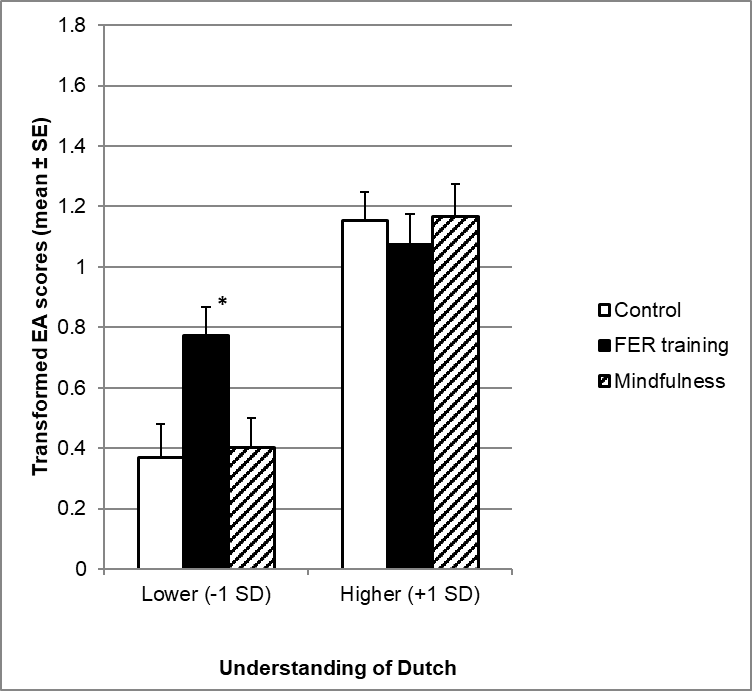
\includegraphics[width=\linewidth]{media/image1.png}

            \caption{}

            \label{fig:rId12}


        \end{figure}
        
Note. *p<0.0083 (comparison with control intervention). EA = Empathic accuracy. FER = facial emotion recognition. SD = standard deviation. SE = standard error.
\end{document}
